\chapter{視覚的特徴の獲得を分析するためのデータセット}
\label{chap:experiment_settings}
本章では,深層学習における,視覚的特徴の獲得メカニズムを紐解くためのデータセットを提案し,その設定の理由と目的と述べる.
これまでの研究では,CNNの学習過程における形状とテクスチャという特徴の獲得と二重降下現象の関係について研究されてきた.
しかし,本研究では形状とテクスチャではなく,色と数字という概念を設定し,2つの学習過程における概念獲得の過程の観測した.

\section{提案データセットの背景}
従来のCNNの研究では,形状バイアスとテクスチャバイアスの学習過程に焦点が当てられてきた.特に,Islamらの研究では,形状とテクスチャを概念として設定して,
CNNモデルの形状・テクスチャバイアスを定量的に計算する手法を提案している.
また,\UTF{9AD9}橋らの研究により,二重降下現象と形状・テクスチャバイアスの変化のタイミングに相関があることが示されている.
しかし,形状やテクスチャという概念は,データセットから帰納的に定められるものであり,正確に定義することが難しく,より詳細な分析を行うことが困難である.
また,CNNが獲得する視覚的特徴は形状やテクスチャに限らず,より基本的な概念,例えば色や数字といった要素も重要な学習対象となる.
これらの基本的な概念の獲得過程を理解することは,CNNの学習メカニズムの解明に新たな知見をもたらす可能性がある.
そこで,今回の提案するデータセットに関しては,目的である学習過程の概念獲得の分析ということを考え,新たに作成したデータセットを作成するうえで3つの条件を
設定した.

\begin{itemize}
    \item 直感的な概念
    \item 2つの概念が独立
    \item 難易度の操作が可能
\end{itemize}

それぞれの条件を設定した理由について以下に述べる.

\subsection{直感的な概念}
形状やテクスチャの概念は,人間が直感的に理解できる概念であるため,これらの概念を用いた研究が多く行われてきた.
しかし,形状やテクスチャといった概念は,データセットから帰納的に定められるものであり,正確に定義することが難しい.
そのため,より直感的な概念を設定することで,より詳細な分析を行うことが可能となる.

\subsection{2つの概念が独立}
形状やテクスチャの概念は,一般に独立ではないため,これらの概念を用いた研究では,概念間の相互作用を考慮する必要がある.
しかし,概念間の相互作用を考慮することは,分析を複雑化させるため,より独立な概念を設定することで,より詳細な分析を行うことが可能となる.

\subsection{難易度の操作が可能}
形状やテクスチャの概念は,難易度の操作が難しいため,これらの概念を用いた研究では,難易度の操作が困難である.
しかし,難易度の操作が可能な概念を設定することで,より詳細な分析を行うことが可能となる.
例えば、片方の概念を固定し,もう一方を難易度操作したときの学習過程を分析すると,相互作用の影響がないことを示すことができ,独立であることを示すことができる.
また,片方の概念を固定し,もう一方を難易度操作して,学習の難易度に差をつけることで,学習過程の難易度による変化を分析することができる.

\newpage

\section{提案するデータセット:Colored EMNIST}
本研究では,バランス調整されたEMNIST Digitsデータセット(数字0-9の10クラス)\cite{cohen2017emnist}を基にカスタムデータセットを作成した.
NIST Special Database 19から抽出・加工されたサブセットである.
このカスタムデータセットは総画像数280,000枚で構成され,そのうち240,000枚が訓練データ,40,000枚がテストデータとして使用される.
各クラスのデータ数はすべて同じであり,訓練データでは各クラス2,400枚,テストデータでは各クラス400枚が含まれる.
元の画像サイズは28x28ピクセルのグレースケール画像だが,最終的にはResNet18の入力に合わせて32x32ピクセルにリサイズした.
具体的には,以下の手順でデータセットを構築した:

\begin{enumerate}
    \item EMNIST Digitsデータセットの各数字クラスのデータを10分割し,それぞれに色概念を付与する.
    \item 色の選択には,3次元RGB空間にランダムに10,000点をプロットし,k-means法により10クラスターを生成する.
    \item 各クラスターの中心座標を代表RGB値として採用する.これにより,色クラスの特徴空間を均等に配置し,人為的なバイアスを排除する.クラス代表間の平均距離は162.4,標準偏差は40.7であった.
    \item データ$x$に付与された色概念を$C_i$とするとき,3次元正規分布$N(\mu_i, \sigma^2)$からサンプリングされた3次元ベクトルを$x$のRGB値とする.
\end{enumerate}
色クラスの特徴空間を図\ref{fig:DistributionColors}に示す.
また,それぞれのクラス間距離を表\ref{fig:color_class_distance}に示す.
そして,図\ref{fig:ColoredEMNIST}に各クラスの画像例の一覧を示す.
このデータセット設計により,合計100クラス(数字10クラス × 色10クラス)の分類タスクを実現した.

\begin{figure}[H]
    \centering
    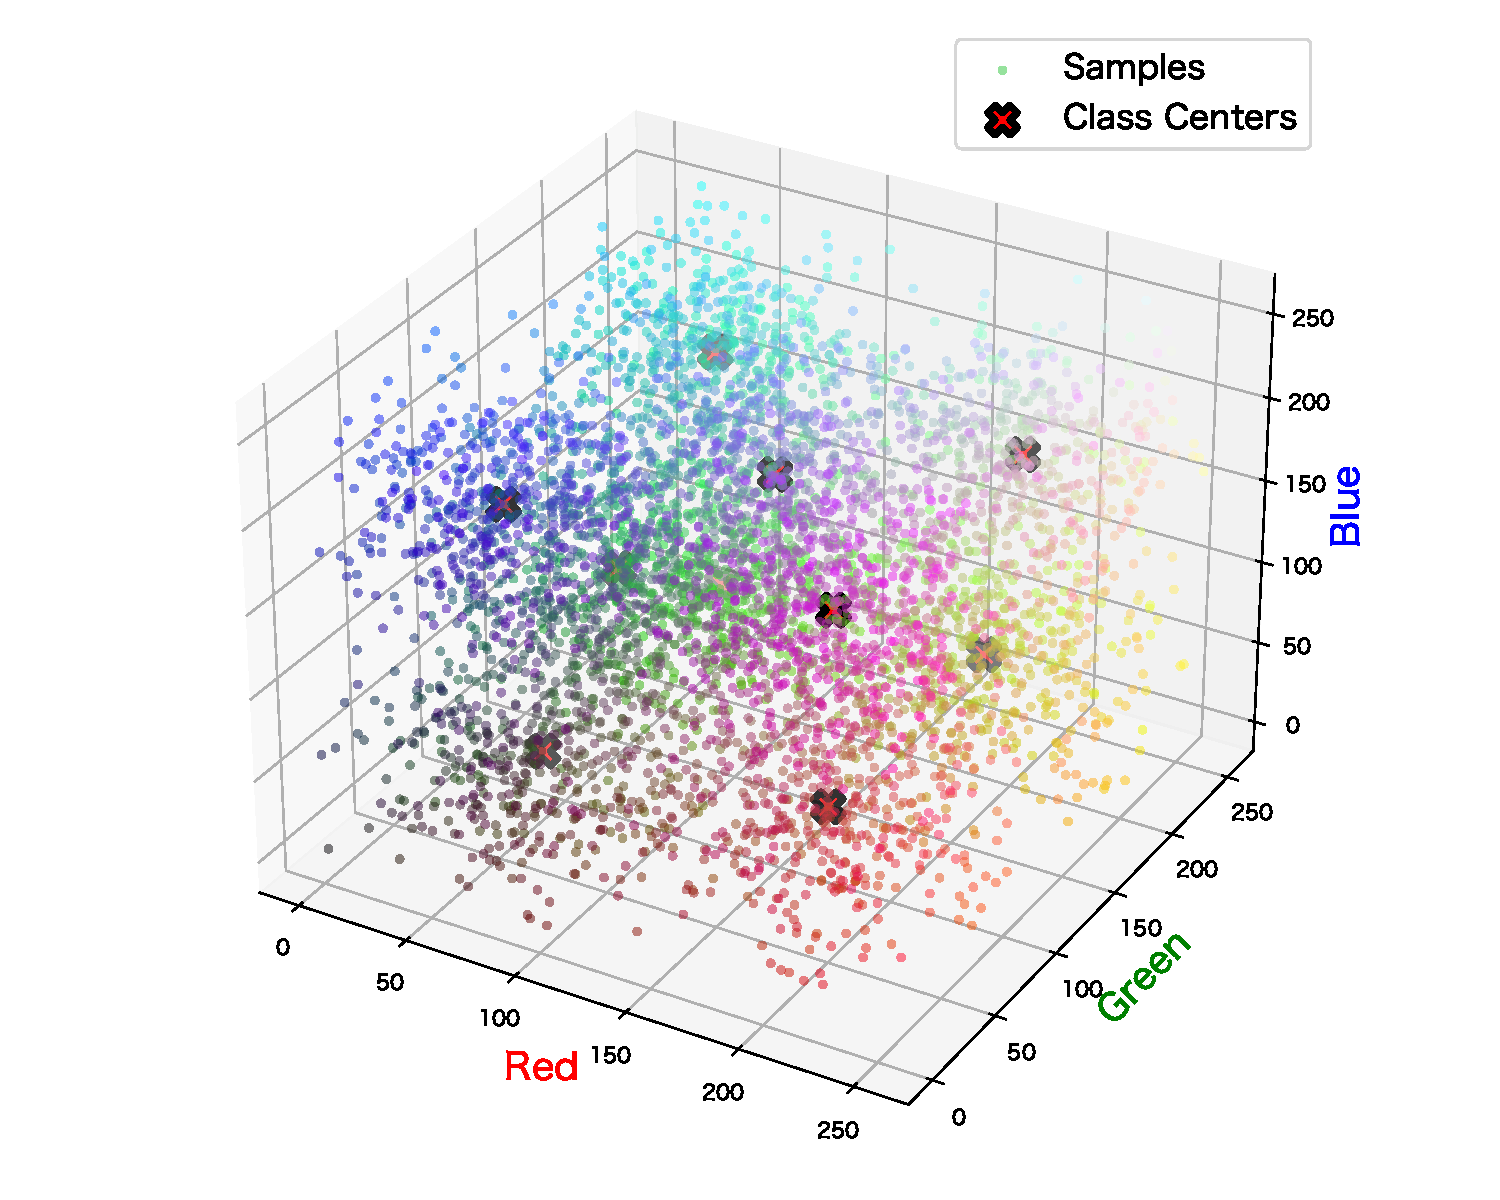
\includegraphics[width=1\columnwidth]{fig/DistributionColors.pdf}
    \caption[RGB色空間における10種類の色クラスの分布を示した3次元散布図]{
        RGB色空間における10種類の色クラスの分布を示した3次元散布図.
        各色クラスはk-means法を用いて均等に分布するよう決定されており,各クラスの中心が赤い「X」マーカーで強調表示されている.
        これにより,色クラス間の平均距離がほぼ均等となり,色概念の識別が均一に行えるような条件が設定されている.
        周囲の点はそれぞれのクラス中心を基準に生成されたサンプルを表し,適度なばらつきを持ちながらも,
        クラス間の明確な分離が保たれている.
    }
    \label{fig:DistributionColors}
\end{figure}

\begin{figure}[H]
    \centering
    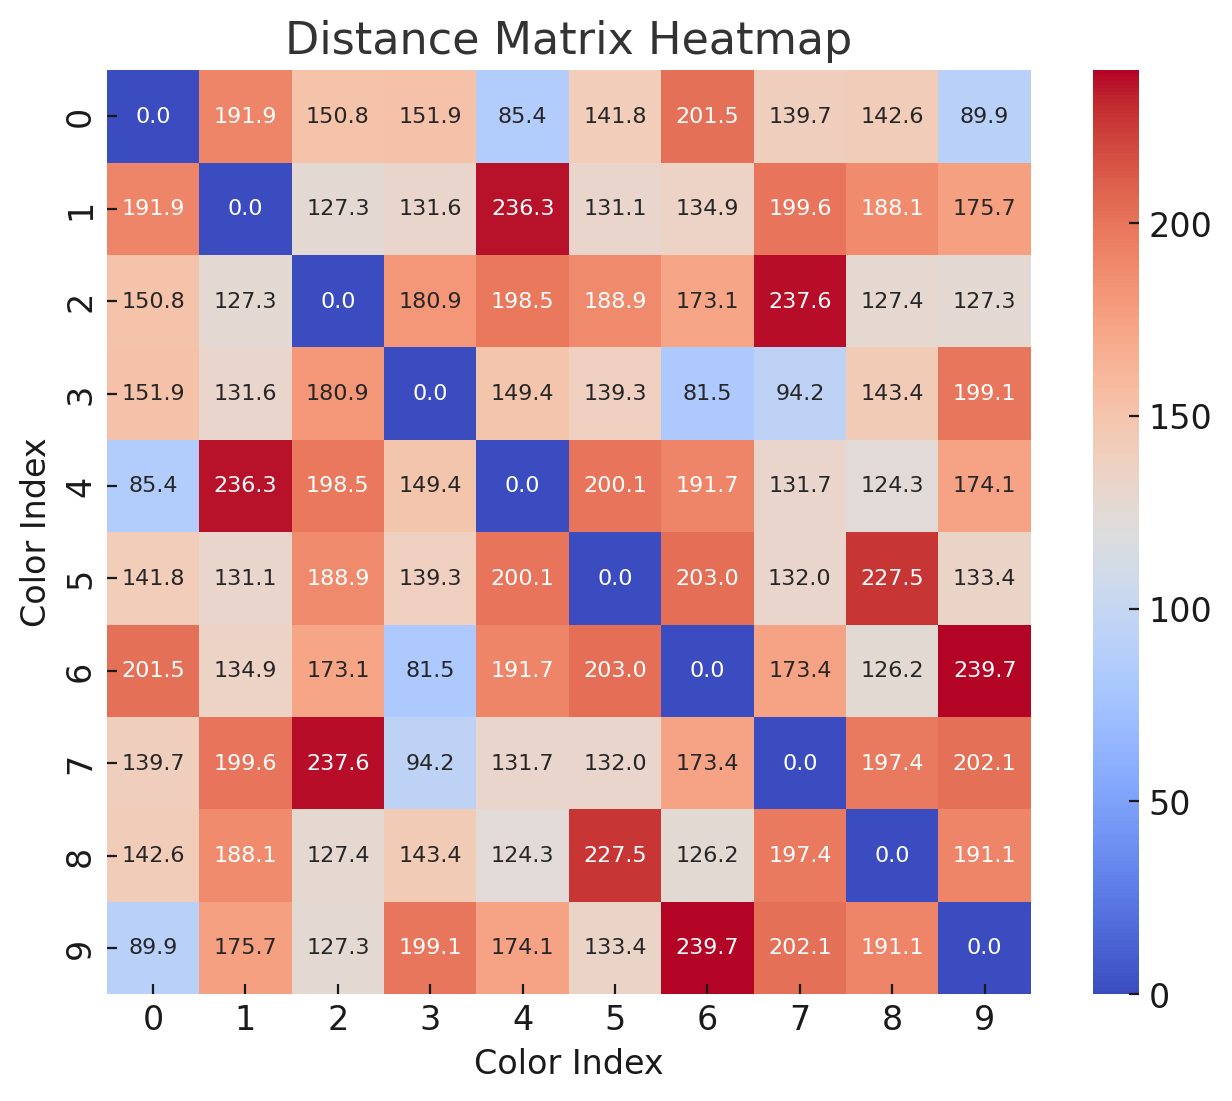
\includegraphics[width=\columnwidth]{tables/Distance_Matrix_Heatmap_color.png}
    \caption[色クラス間の平均距離を示すヒートマップ]{
        色クラス間の平均距離を示すヒートマップ.
        各セルは,対応する色クラス間の平均距離を示しており,色クラス間の距離が均等に分布していることが確認できる.
    }
    \label{fig:color_class_distance}
\end{figure}

\begin{figure}[H]
    \centering
    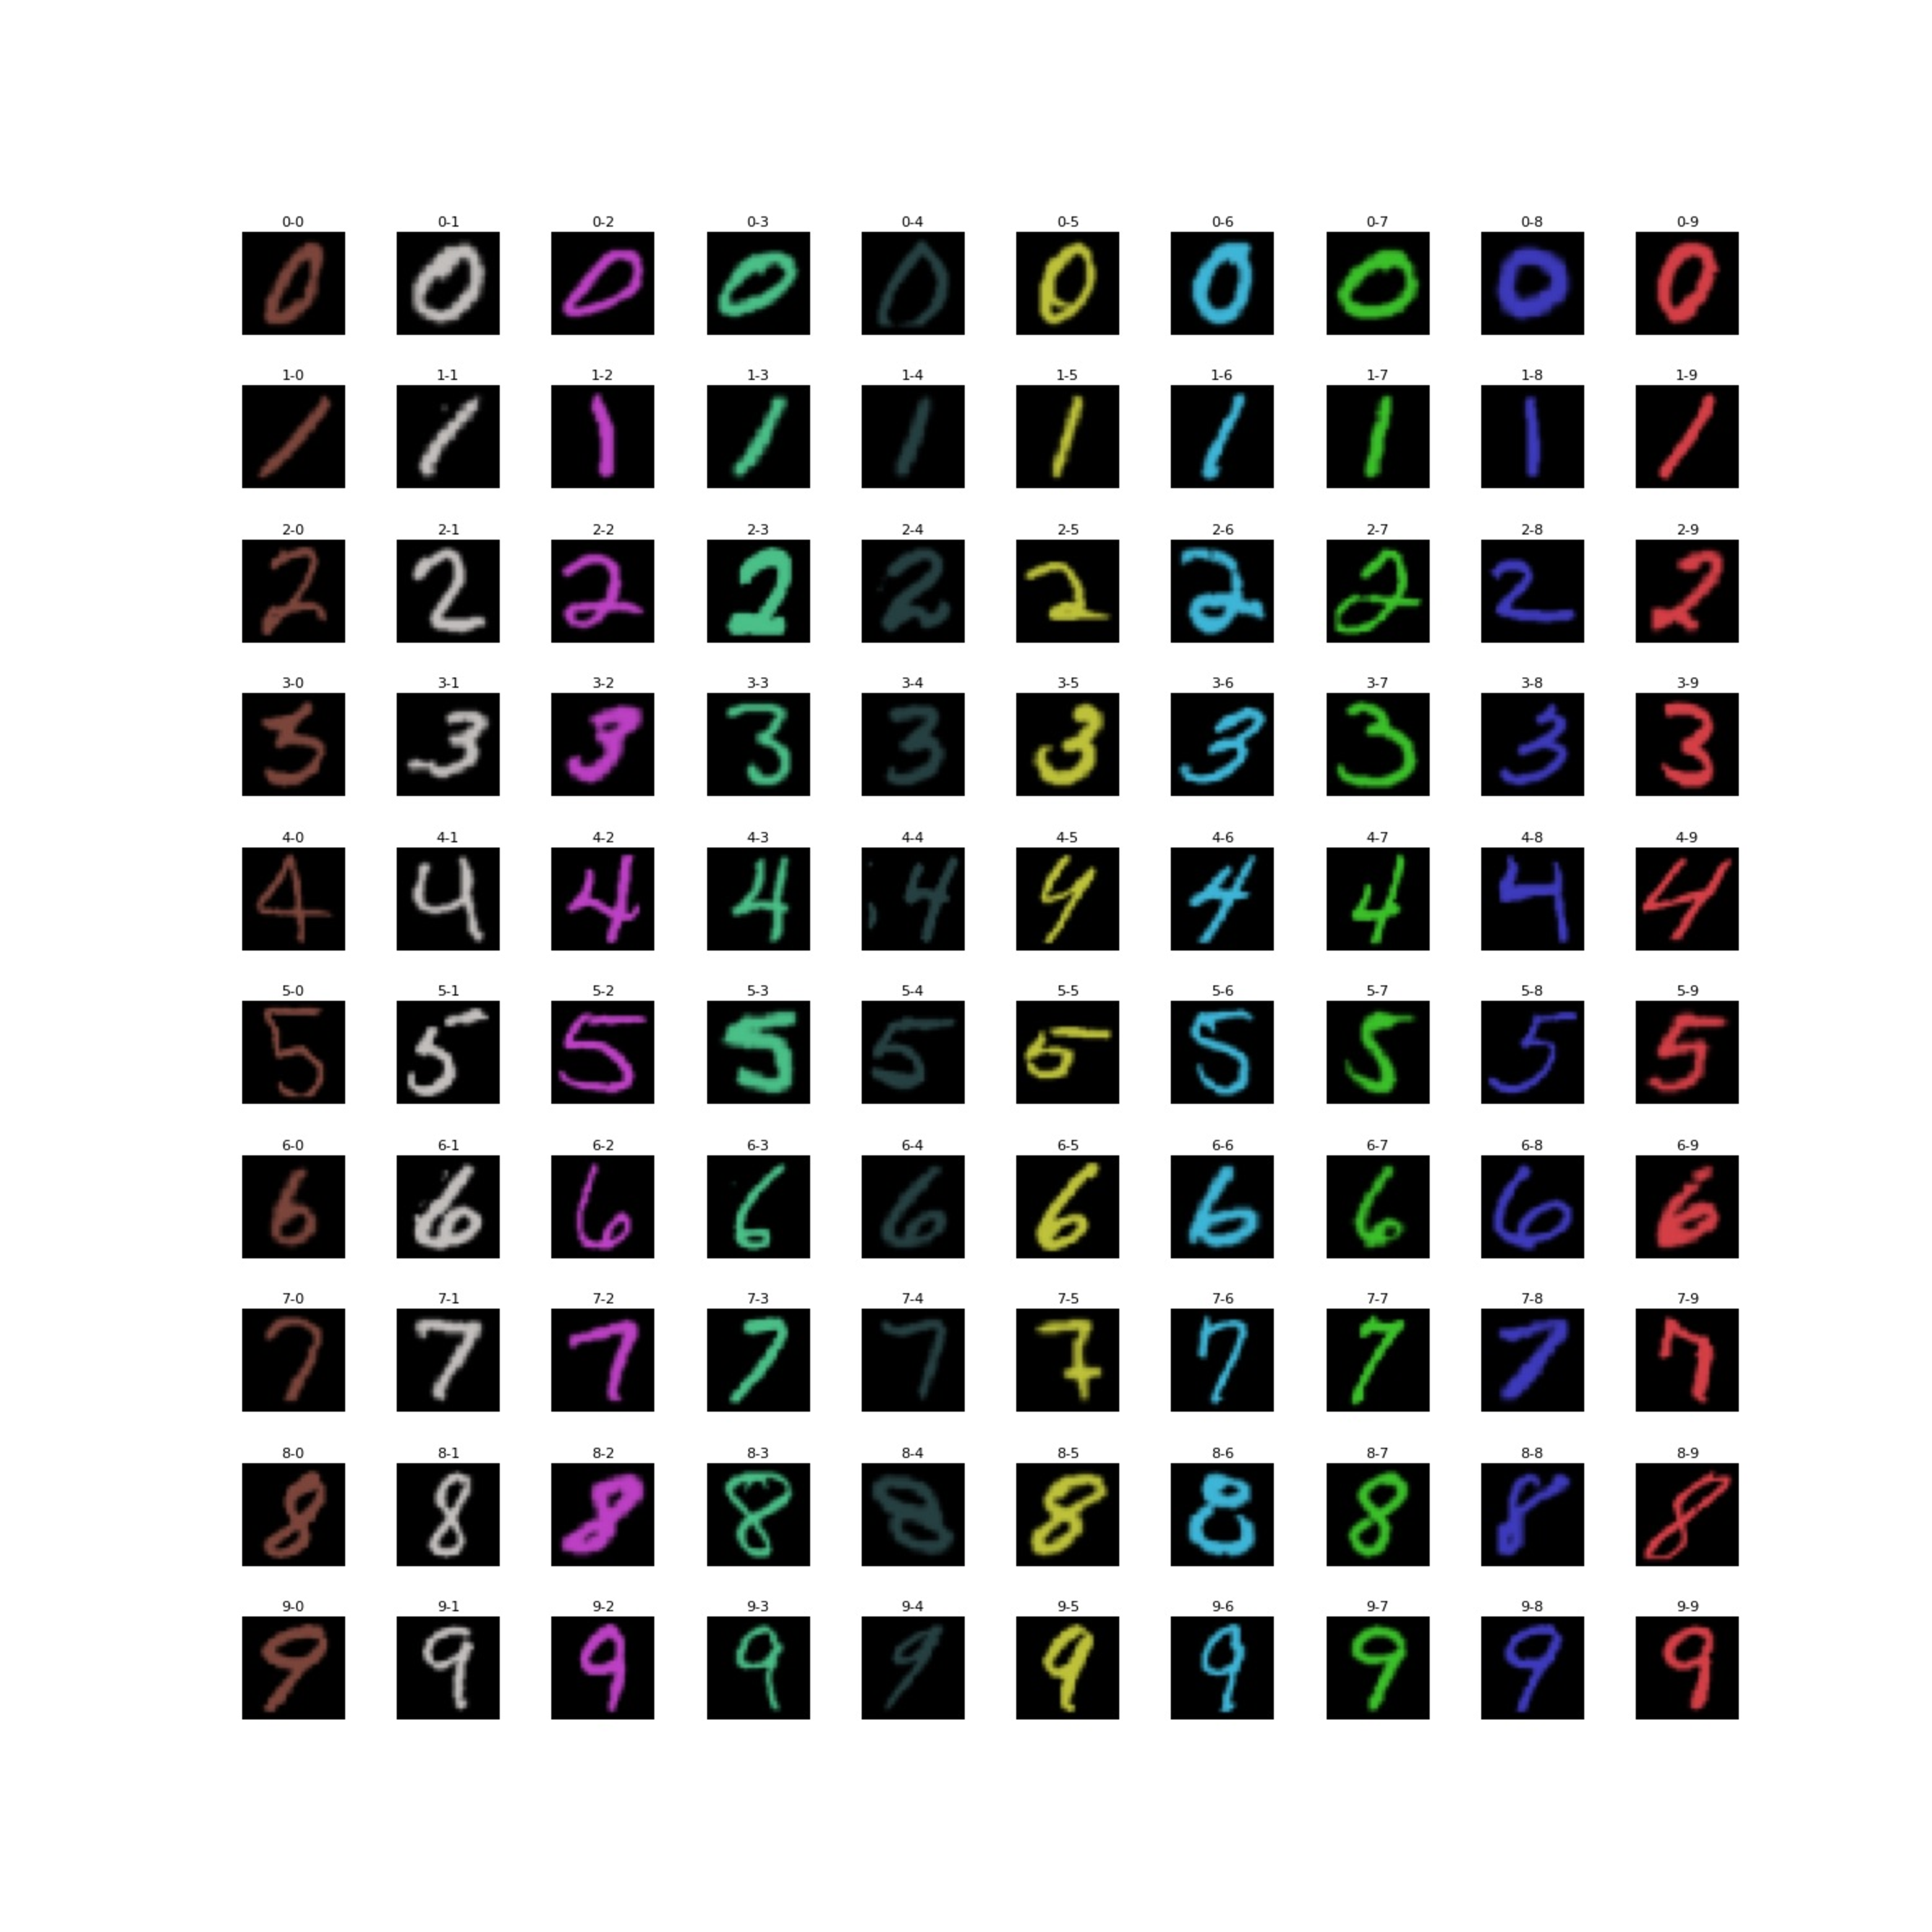
\includegraphics[width=1\columnwidth]{fig/coloredemnist_0.pdf}
    \caption[Colored EMNISTデータセットの画像例]{
        Colored EMNISTデータセットの画像例.
        各数字クラス(0-9)に対して,10種類の色クラスがランダムに割り当てられている.
        このデータセットは,数字と色の概念を組み合わせた合計100クラスの分類タスクを提供する.
        行が数字クラス,列が色クラスを示しており,各セルは数字クラスと色クラスの組み合わせに対応する画像を示している.
    }
    \label{fig:ColoredEMNIST}
\end{figure}

\newpage

\section{色概念における難易度調整手法}
色概念の難易度は,RGB値のばらつきを示すパラメータ$\sigma^2$によって制御される.
この手法には以下の特徴がある:$\sigma^2$はすべての色クラスで一定とし,3次元空間でバランスの取れた色分布を実現する.
色概念間の識別に関するBayes errorを$\sigma^2$によって制御することが可能である.
$\sigma = 0$の場合,代表RGB値のみが付与される.$\sigma^2 = 10^3, 10^{3.5}, 10^4$では,
色クラスの分布がより広がり,色概念の識別がより困難になる.
図\ref{fig:coloredeminsts}に,$\sigma^2 = 0, 10^3, 10^{3.5}, 10^4$の場合の画像例を示す.

\begin{figure}[H]
    \centering
    \begin{subfigure}[b]{0.48\textwidth}
        \centering
        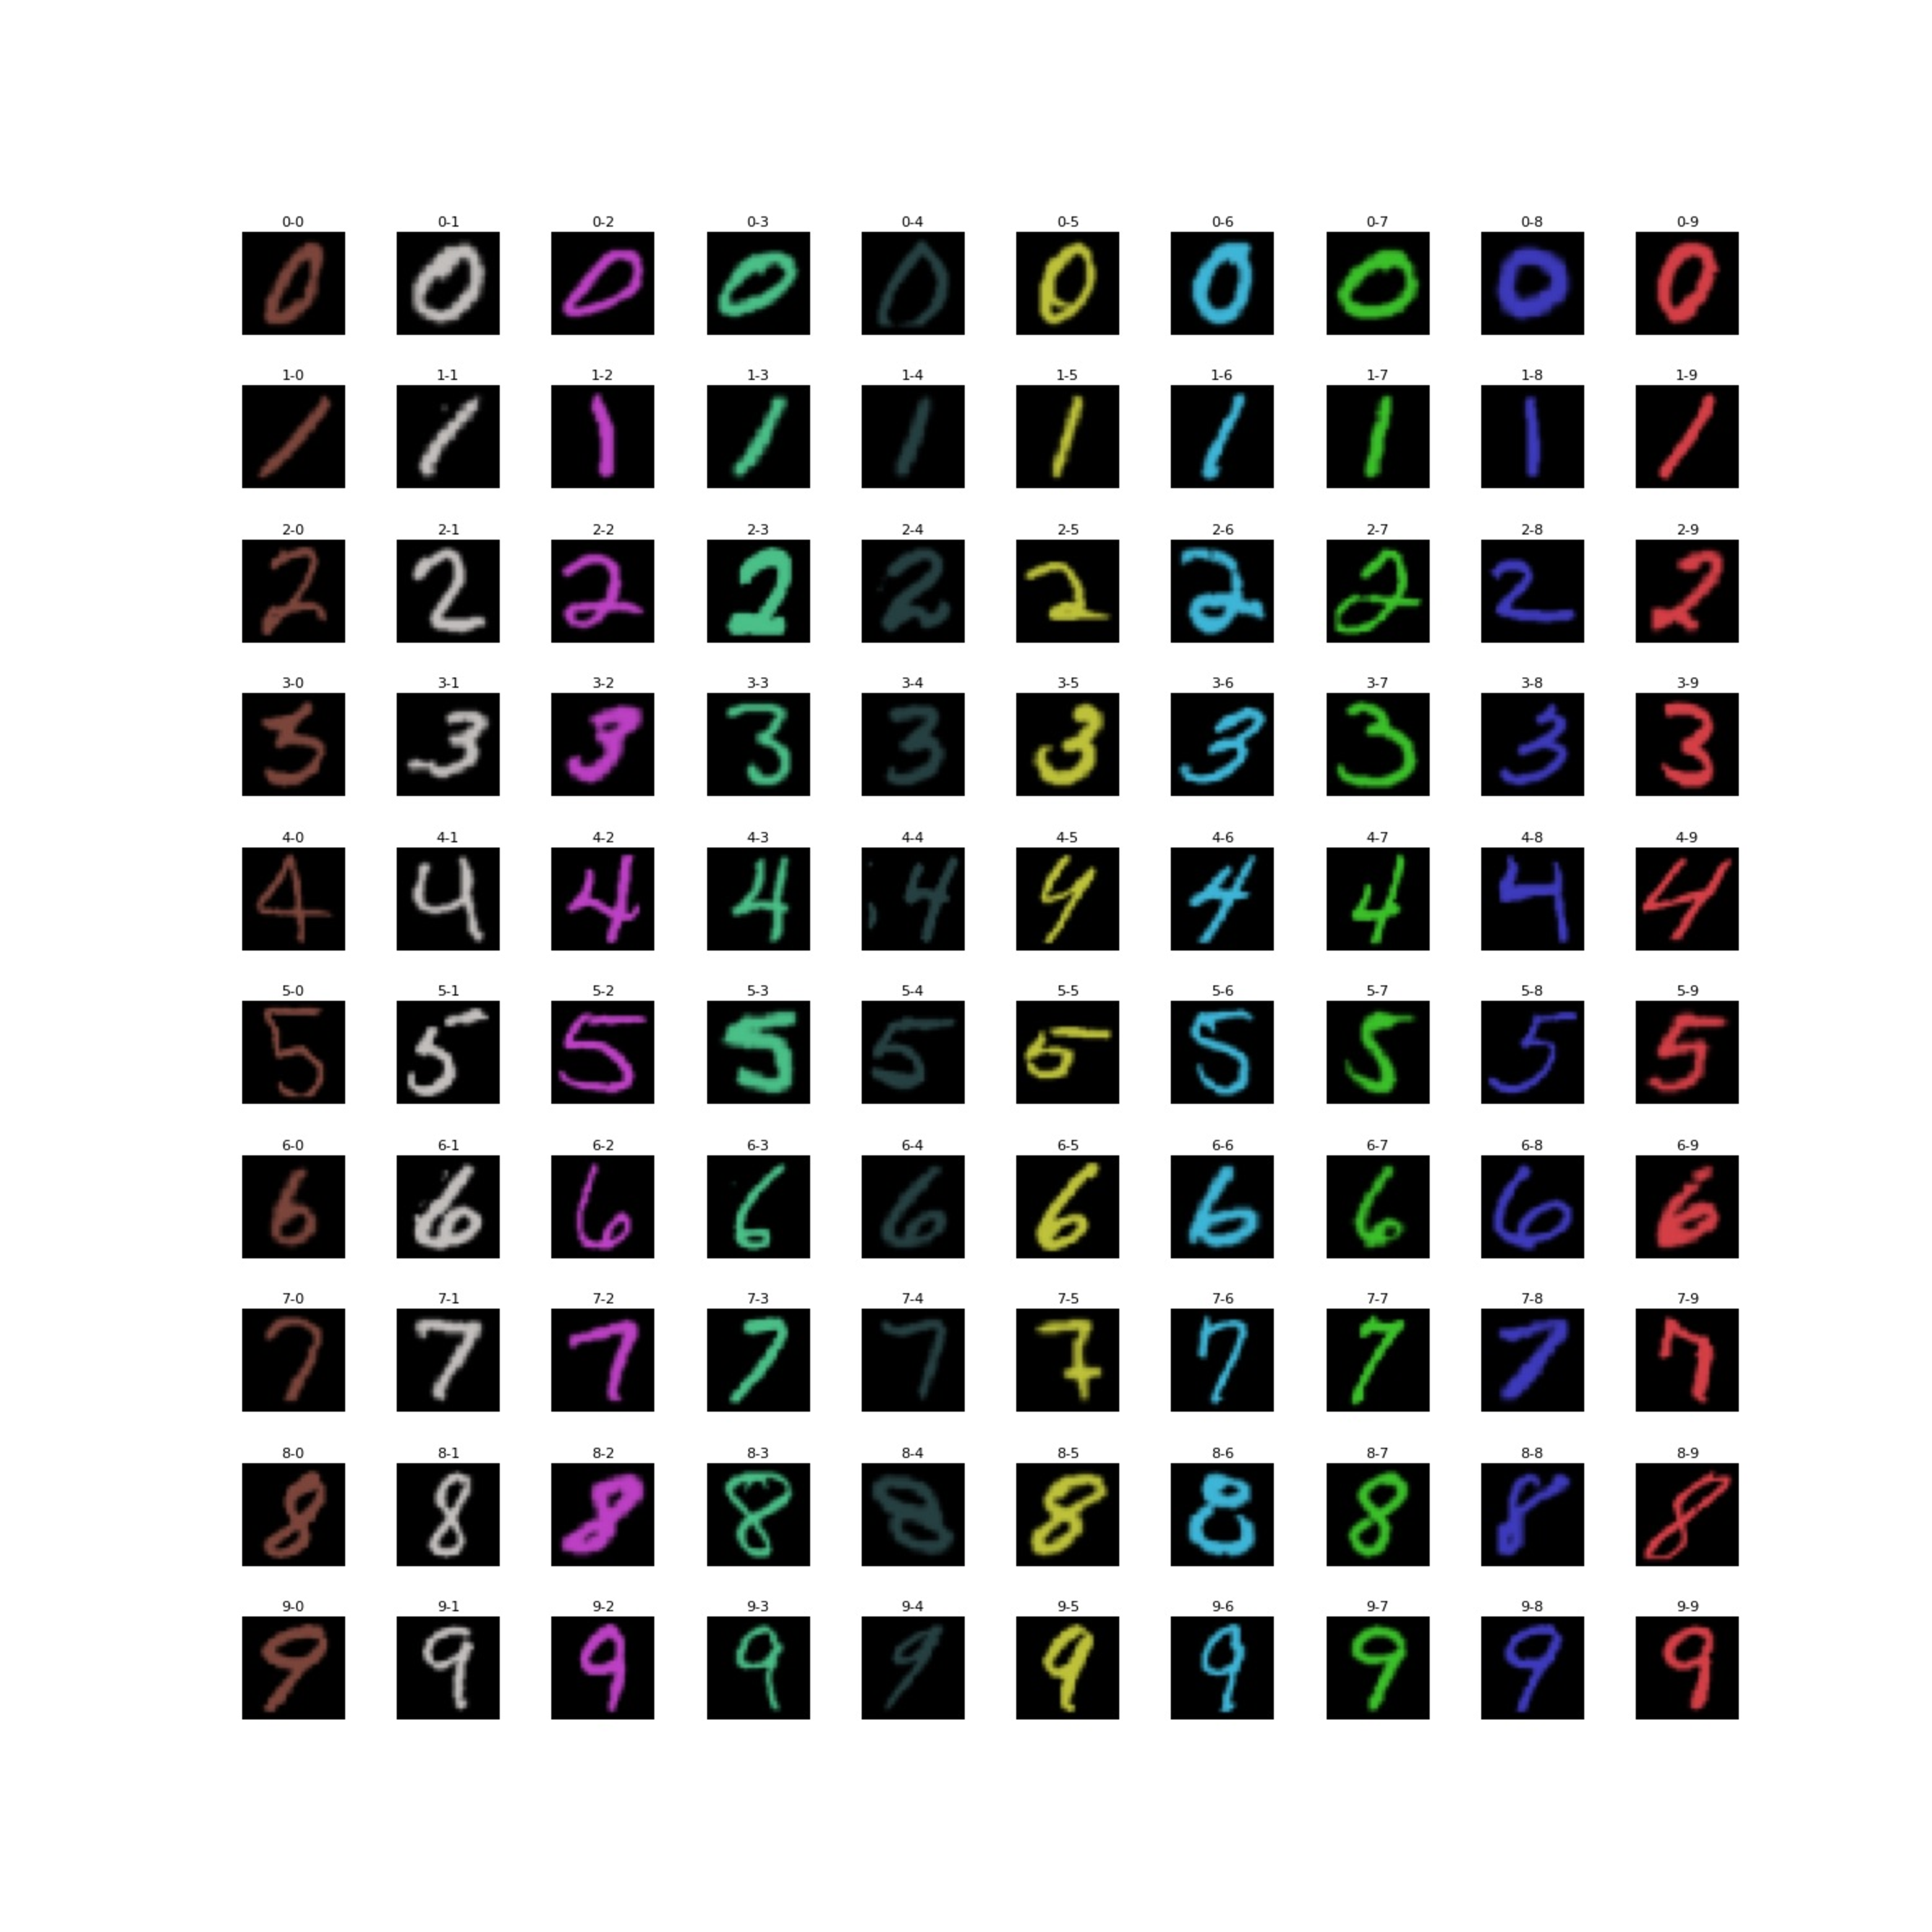
\includegraphics[width=\textwidth]{fig/coloredemnist_0.pdf}
        \caption{$\sigma^2 = 0$}
        \label{fig:coloredeminst_0}
    \end{subfigure}
    \hfill
    \begin{subfigure}[b]{0.48\textwidth}
        \centering
        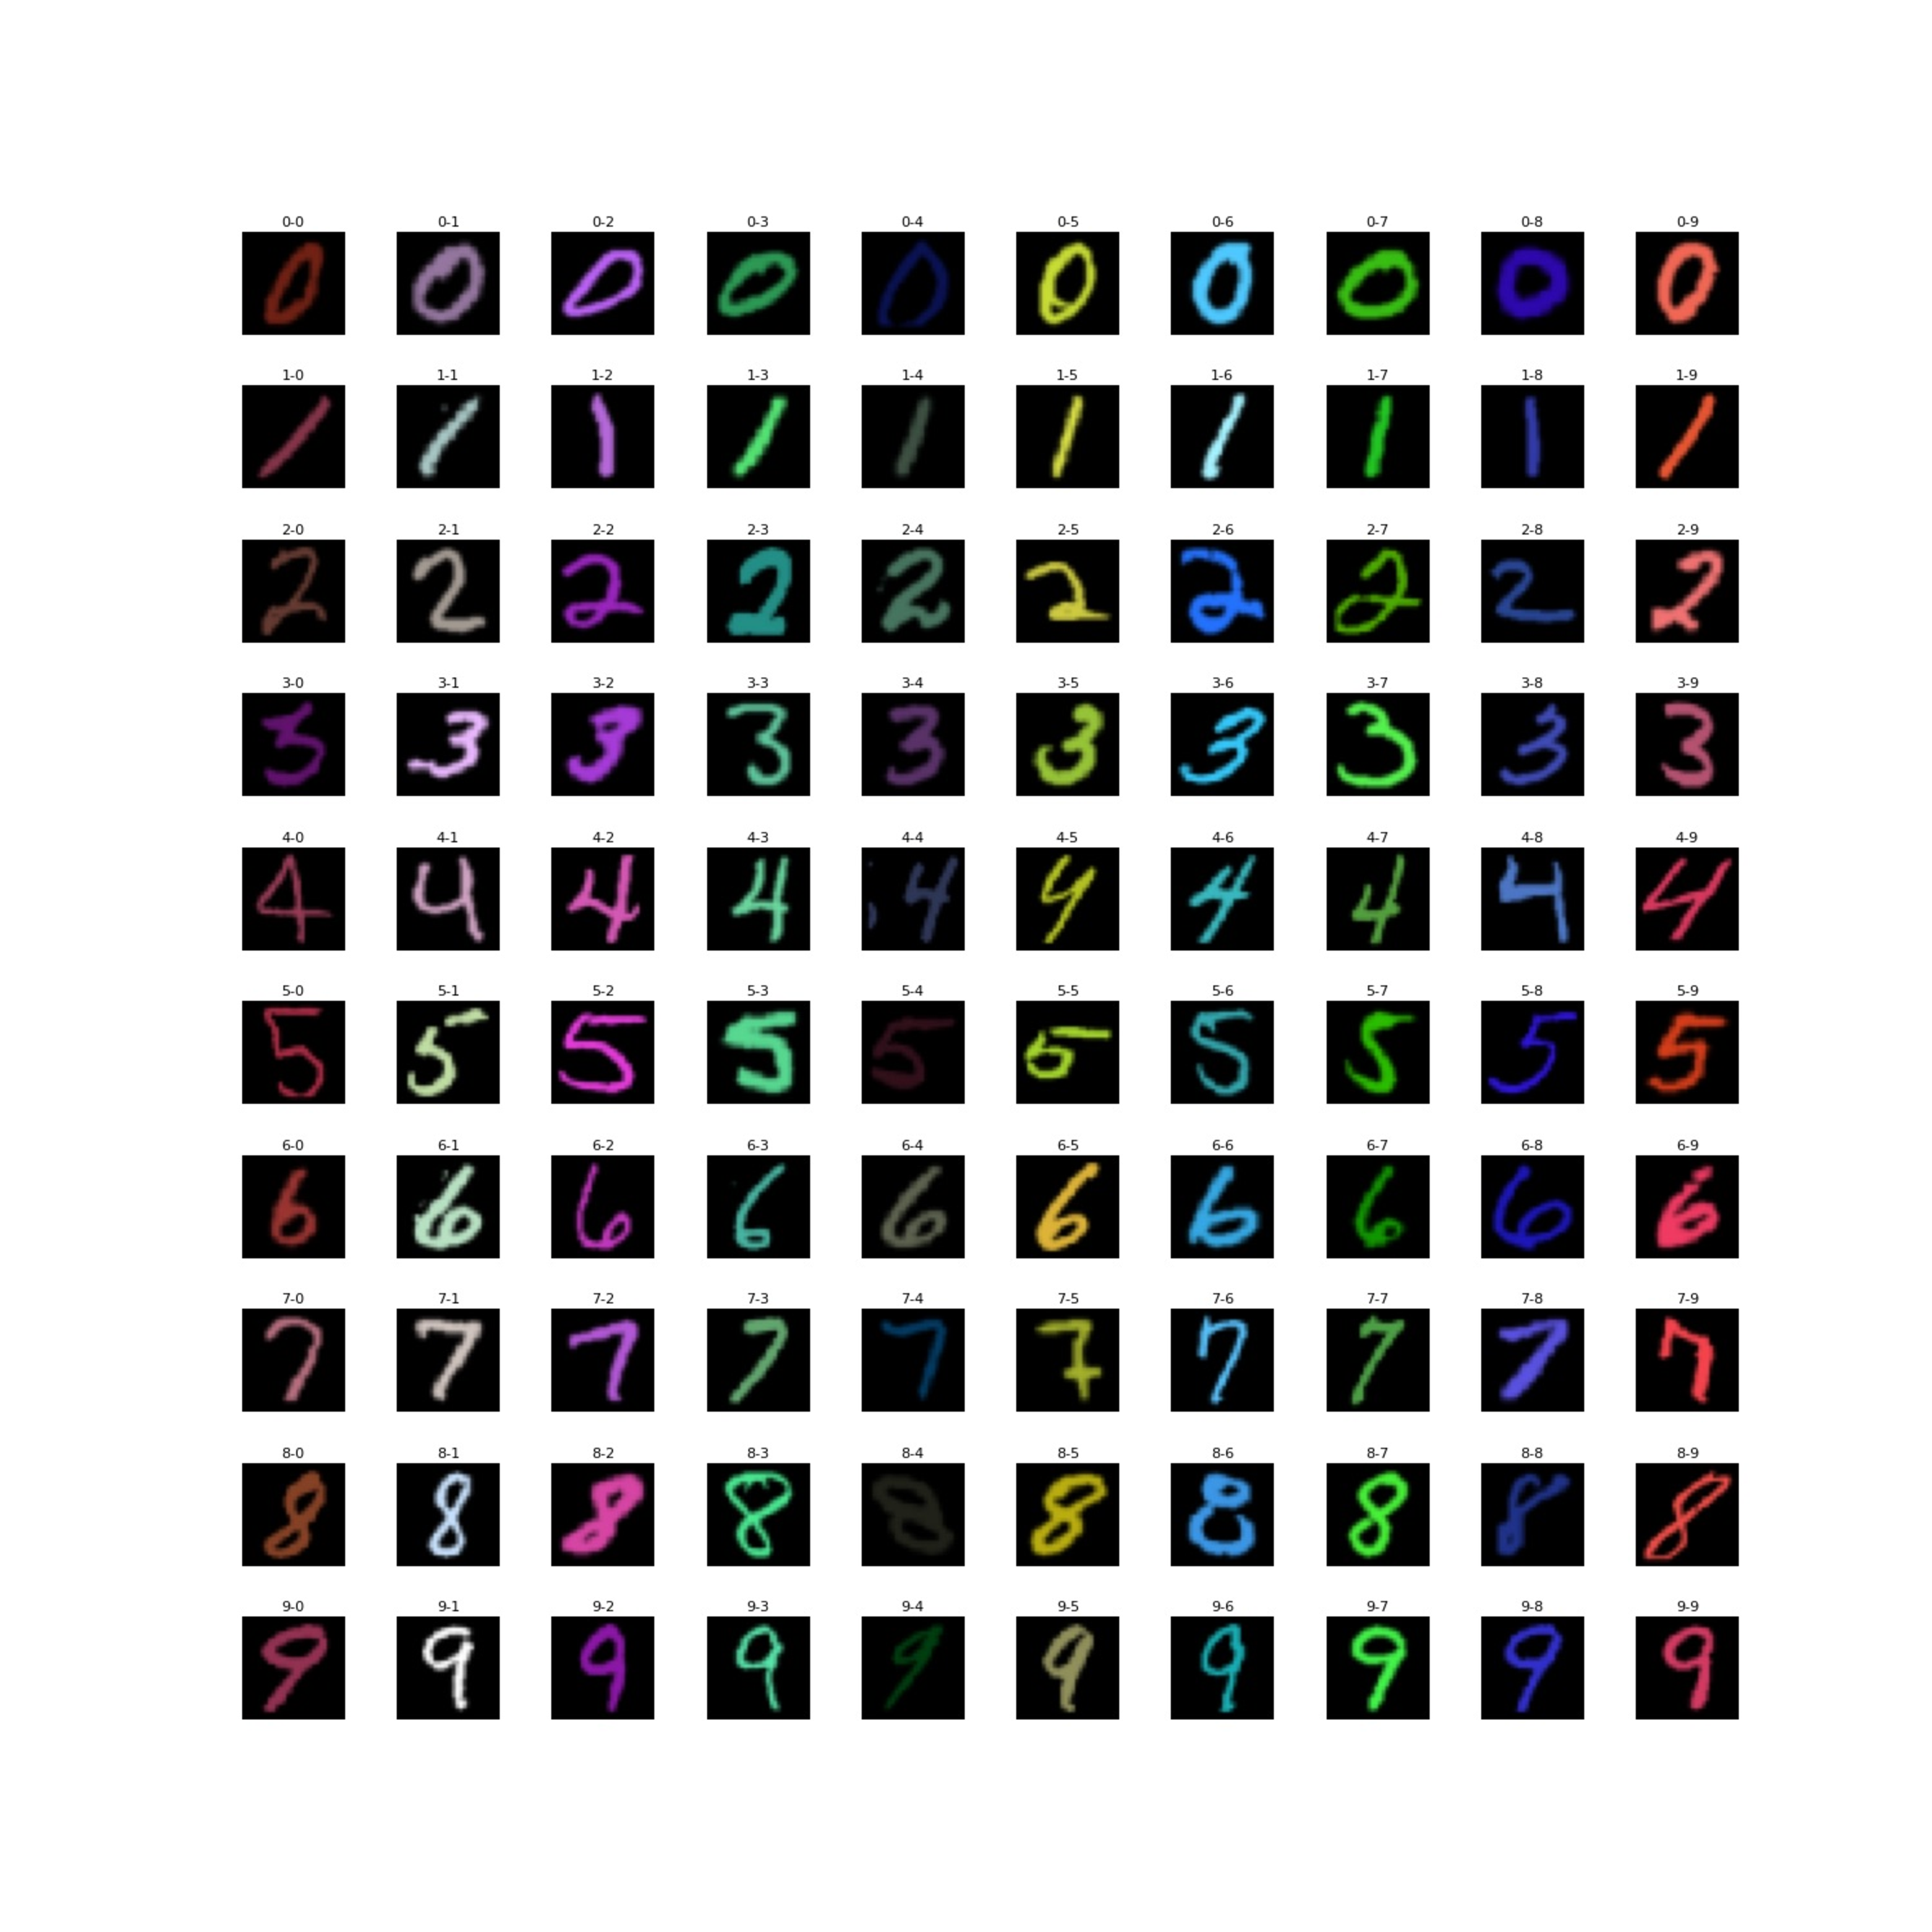
\includegraphics[width=\textwidth]{fig/coloredemnist_1000.pdf}
        \caption{$\sigma^2 = 10^3$}
        \label{fig:coloredeminst_1000}
    \end{subfigure}
    \vspace{0.5cm}
    \begin{subfigure}[b]{0.48\textwidth}
        \centering
        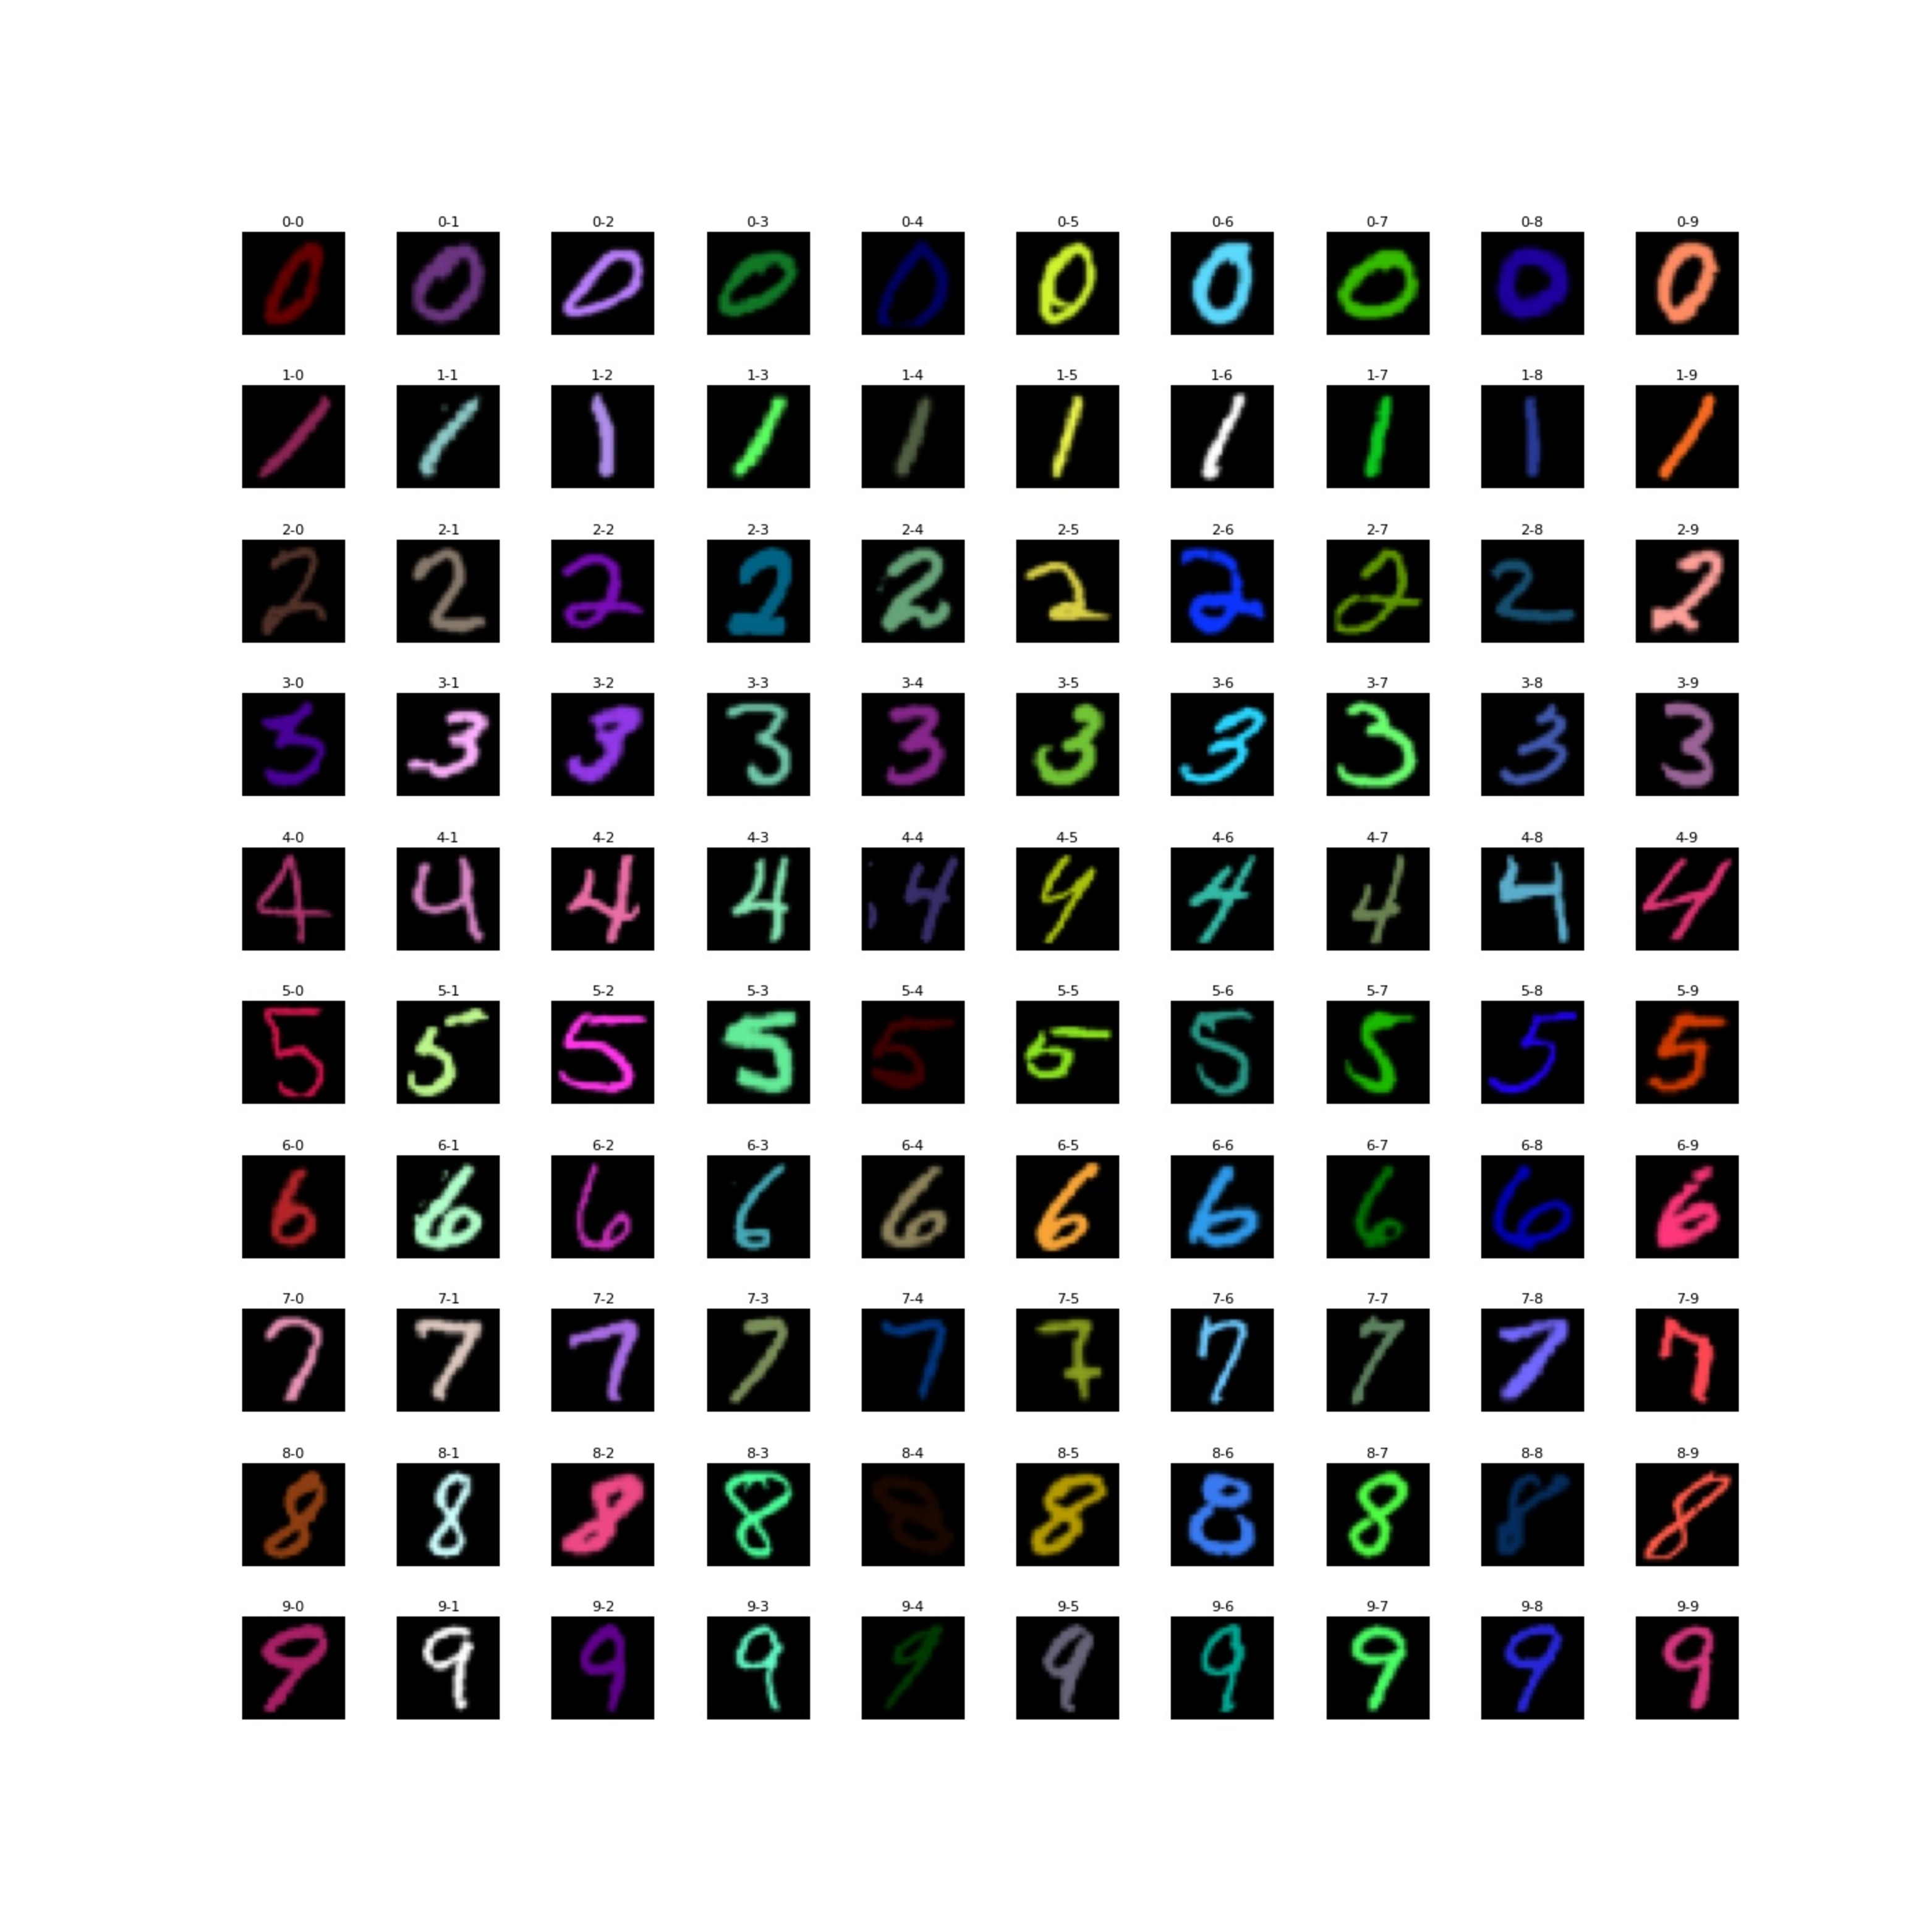
\includegraphics[width=\textwidth]{fig/coloredemnist_3612.pdf}
        \caption{$\sigma^2 = 10^{3.5}$}
        \label{fig:coloredeminst_3612}
    \end{subfigure}
    \hfill
    \begin{subfigure}[b]{0.48\textwidth}
        \centering
        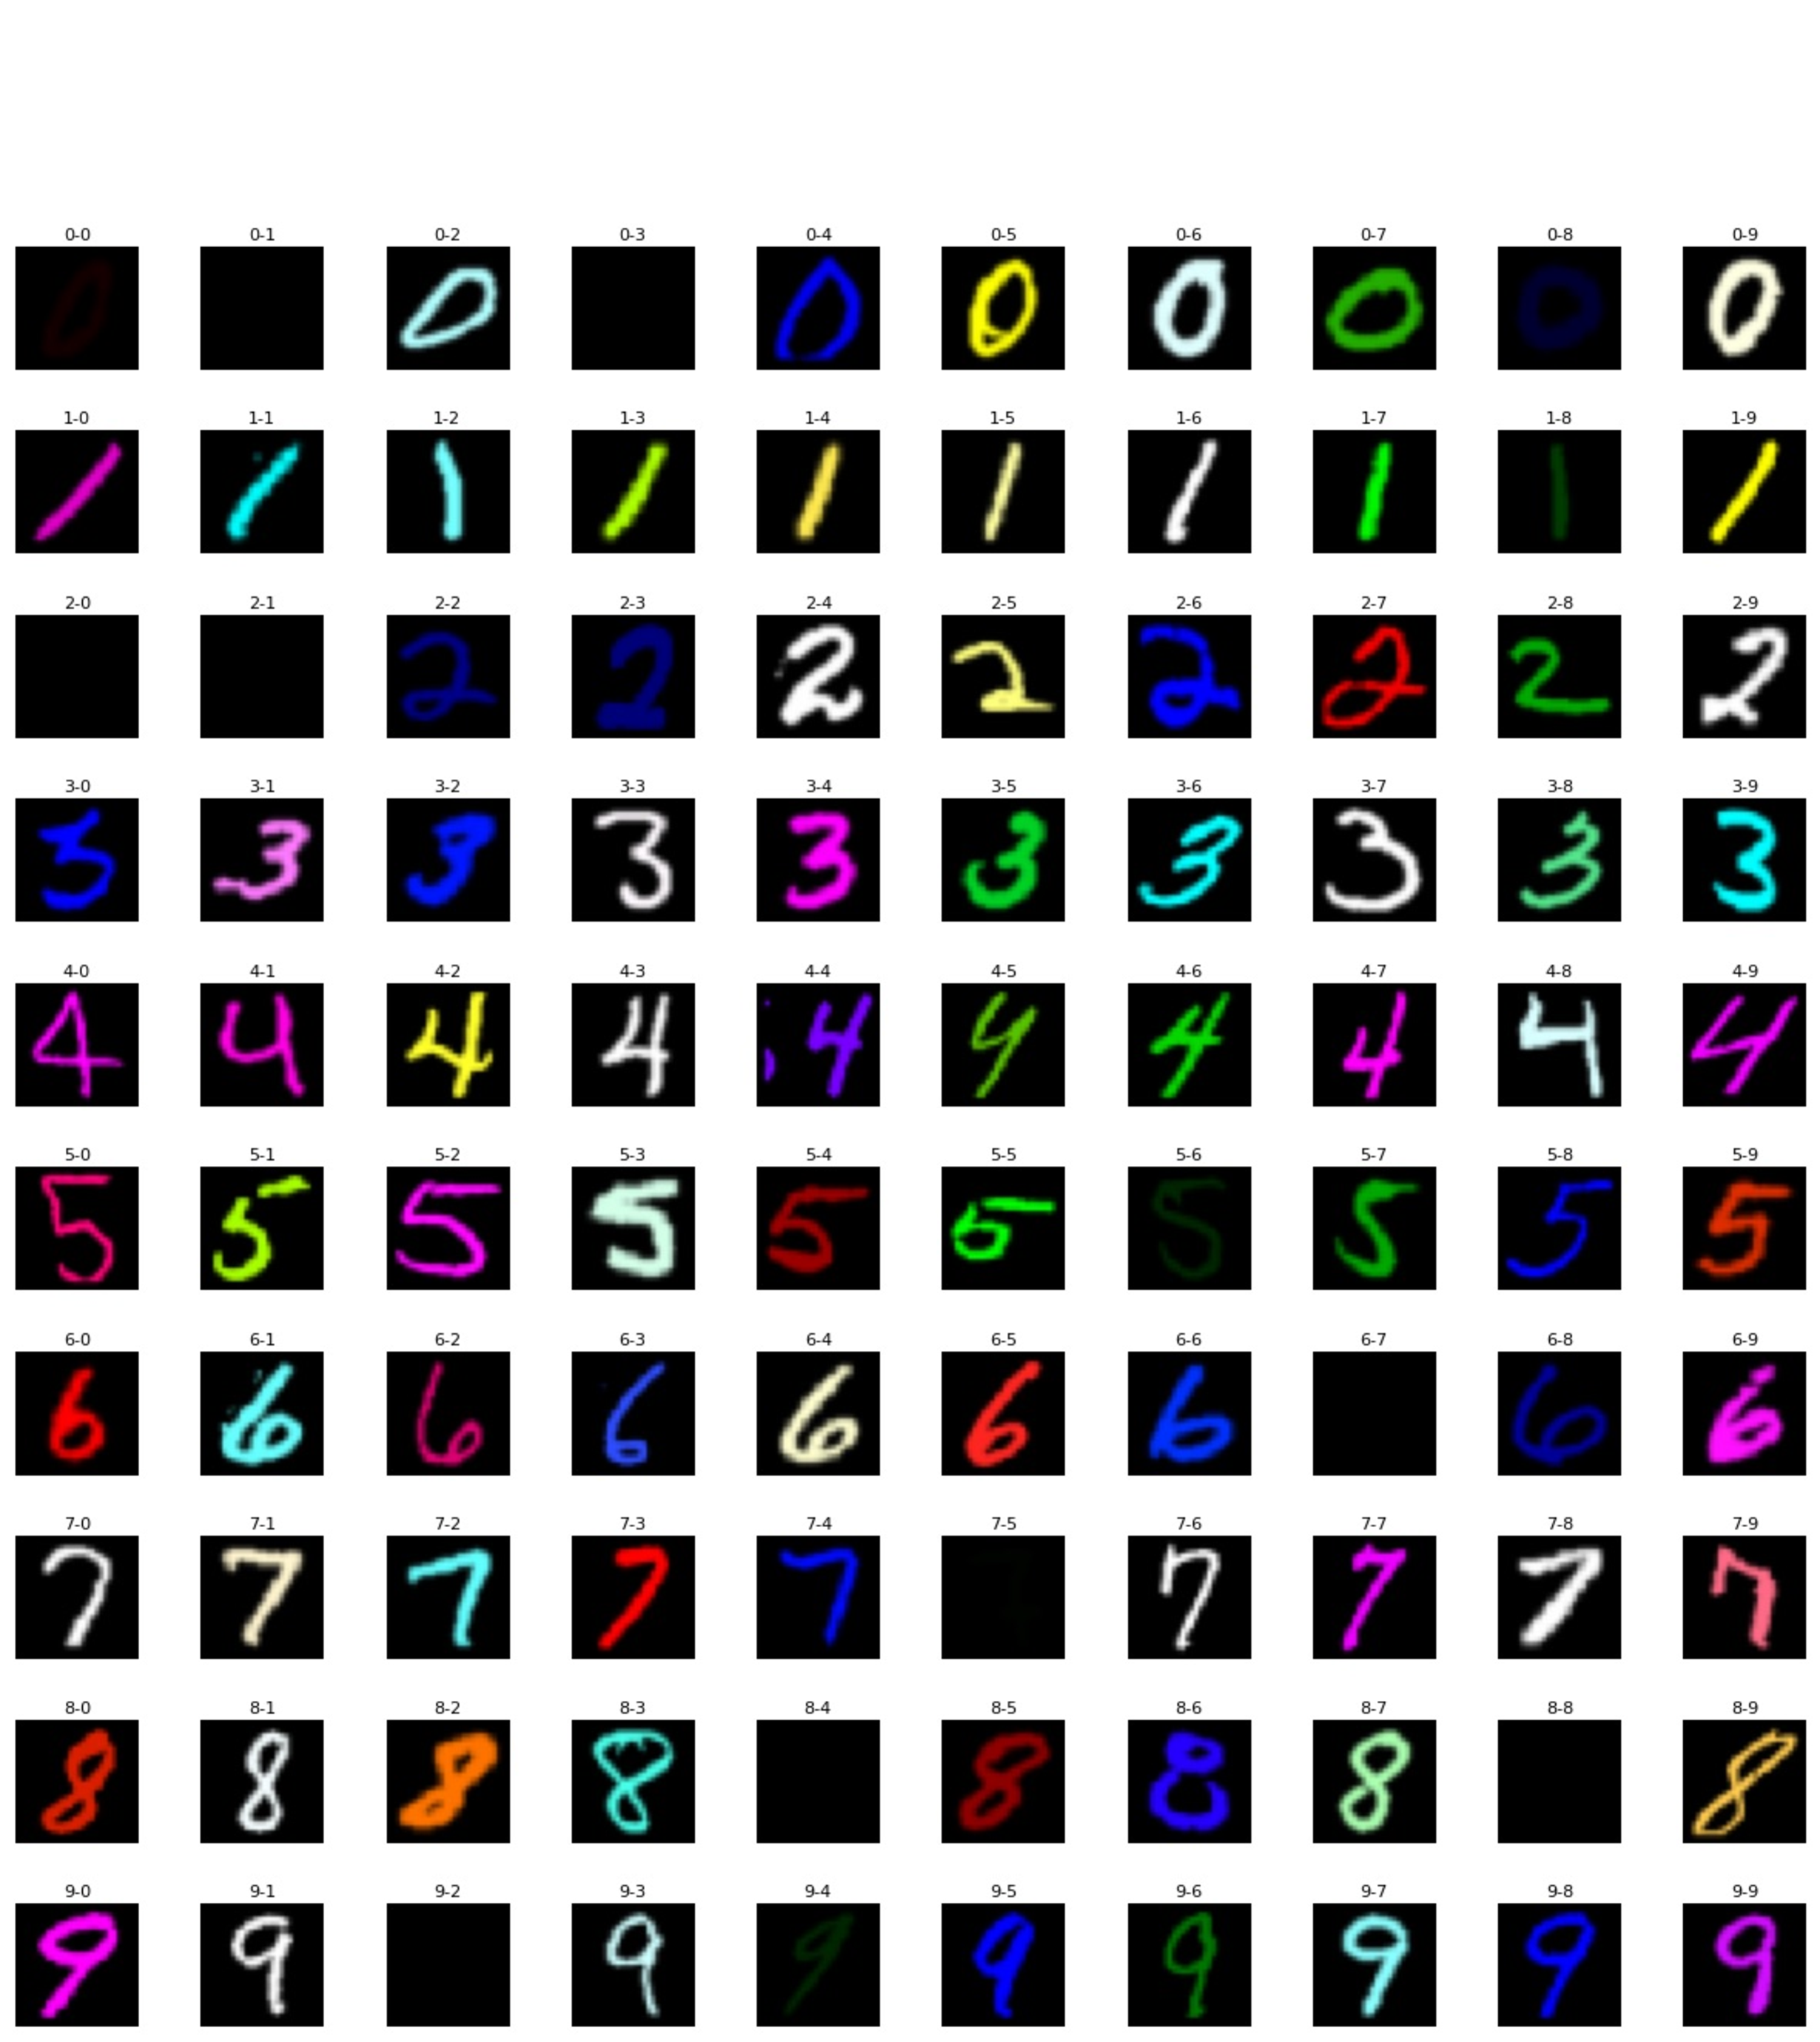
\includegraphics[width=\textwidth]{fig/coloredemnist_10000.pdf}
        \caption{$\sigma^2 = 10^4$}
        \label{fig:coloredeminst_10000}
    \end{subfigure}
    \caption[Colored EMNISTデータセットにおける色概念の難易度調整例]{Colored EMNISTデータセットにおける色概念の難易度調整例.
    100枚の画像において,同じ列が色クラス,行が数字クラスを示している.
    各図は異なるパラメータ$\sigma^2$で生成されたサンプルを示している.$\sigma^2$が増加するにつれて,色概念のばらつきが大きくなる.
    }
    \label{fig:coloredeminsts}
\end{figure}

\section{ラベルノイズの付与}
ラベルノイズは,データセットのラベルに誤りが含まれることを指す.
データセットの品質を低下させる要因の一つであり,機械学習モデルの性能を低下させるほか,二重降下現象を観察するうえで重要な要素である.
本研究では,ラベルノイズを付与することで,モデルのロバスト性や学習効率に関する知見を得ることも目的としている.
ラベルノイズは,各クラスのラベルを一定の確率で別のクラスに置き換えることで実珸される.
ラベルノイズを付与する場合,数字と色のラベルに対してどちらも異なるノイズ率を設定する.
